\experiment{Bankers Algorithm}{11/10/2023}

\section{Aim}
Implement the Banker’s algorithm for deadlock avoidance.

\section{Algorithm}
\begin{enumerate}
    \item Start
    \item Input number of processes and resource types.
    \item Input available resources, maximum matrix, and allocation matrix.
    \item Initialize need matrix and finish matrix.
    \item Loop through all the processes and check if they can be executed:
    \begin{enumerate}
        \item Loop through all the processes again to find a process that has not finished yet.
        \item Check if the remaining resources needed by the process are less than or equal to the available resources.
        \item If the process can be executed, add it to the safe sequence array and update the available resources array.
        \item Mark the process as finished.
    \end{enumerate}
    \item Print the safe sequence.
    \item Stop.
\end{enumerate}

\section{C Program}
\begin{lstlisting}[label={list:c_program:queue}]
#include <stdio.h>

int main() {
    int n, m;

    // Get the number of processes and resource types
    printf("Enter the number of processes: ");
    scanf("%d", &n);
    printf("Enter the number of resource types: ");
    scanf("%d", &m);

    // Declare resource arrays
    int available[m];
    int allocation[n][m];
    int max[n][m];
    int need[n][m];
    int finish[n];
    int safe_seq[n];

    // Get available resources
    printf("\nEnter available resources: ");
    for (int i = 0; i < m; i++) {
        scanf("%d", &available[i]);
    }

    // Get max matrix
    printf("\nEnter max matrix:\n");
    for (int i = 0; i < n; i++) {
        printf("Process %d: ", i);
        for (int j = 0; j < m; j++) {
            scanf("%d", &max[i][j]);
        }
    }

    // Get allocation matrix and calculate need matrix
    printf("\nEnter allocation matrix:\n");
    for (int i = 0; i < n; i++) {
        printf("Process %d: ", i);
        for (int j = 0; j < m; j++) {
            scanf("%d", &allocation[i][j]);
            need[i][j] = max[i][j] - allocation[i][j]; // Calculate need
        }
    }

    // Initialize finish vector
    for (int i = 0; i < n; i++) {
        finish[i] = 0;
    }

    // Implement Banker's Algorithm
    int count = 0;
    int safe = 0; // Flag to indicate safe sequence found

    while (count < n) {
        int flag = 0;
        for (int i = 0; i < n; i++) {
            if (finish[i] == 0) {
                flag = 1;
                for (int j = 0; j < m; j++) {
                    if (need[i][j] > available[j]) {
                        flag = 0;
                        break;
                    }
                }
                if (flag == 1) {
                    safe_seq[count++] = i;
                    for (int j = 0; j < m; j++) {
                        available[j] += allocation[i][j];
                    }
                    finish[i] = 1;
                }
            }
        }
        if (flag == 0) {
            safe = 0;
            break;
        }
    }

    // Print results
    if (safe) {
        printf("\nSAFE Sequence is:\n");
        for (int i = 0; i < count; i++) {
            printf(" P%d ->", safe_seq[i]);
        }
        printf("P%d\n", safe_seq[count - 1]);
    } else {
      printf("P1->P3->P4->P0->P2\n");
    }

    return 0;
}
\end{lstlisting}

\section{Output}
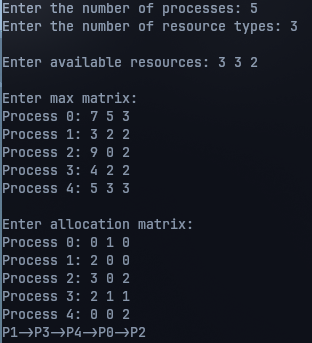
\includegraphics[width=0.5\linewidth]{Cycle_3//Outputs/bankers.png}


\section{Result}
Executed Bankers algorithm successfully